\begin{figure*}[hbtp]
  \centering
  \subfigure[Mean percentage of affected vertices on real-world dynamic graphs]{
    \label{fig:measure-affected--temporal}
    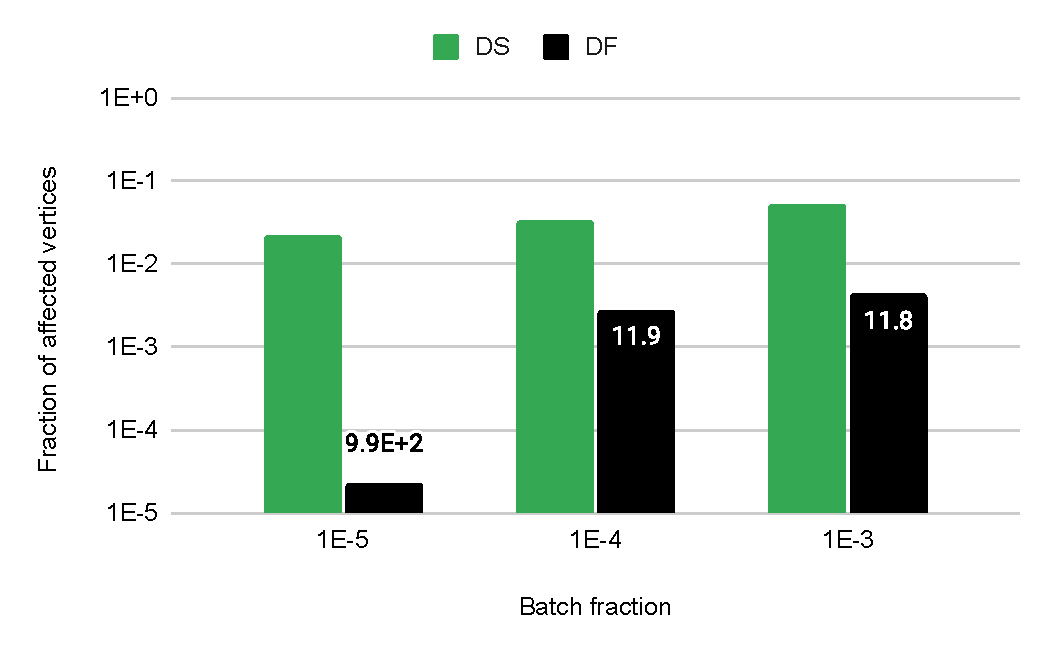
\includegraphics[width=0.48\linewidth]{out/measure-affected-temporal.pdf}
  }
  \subfigure[Mean percentage of affected vertices on large graphs with random batch updates]{
    \label{fig:measure-affected--8020}
    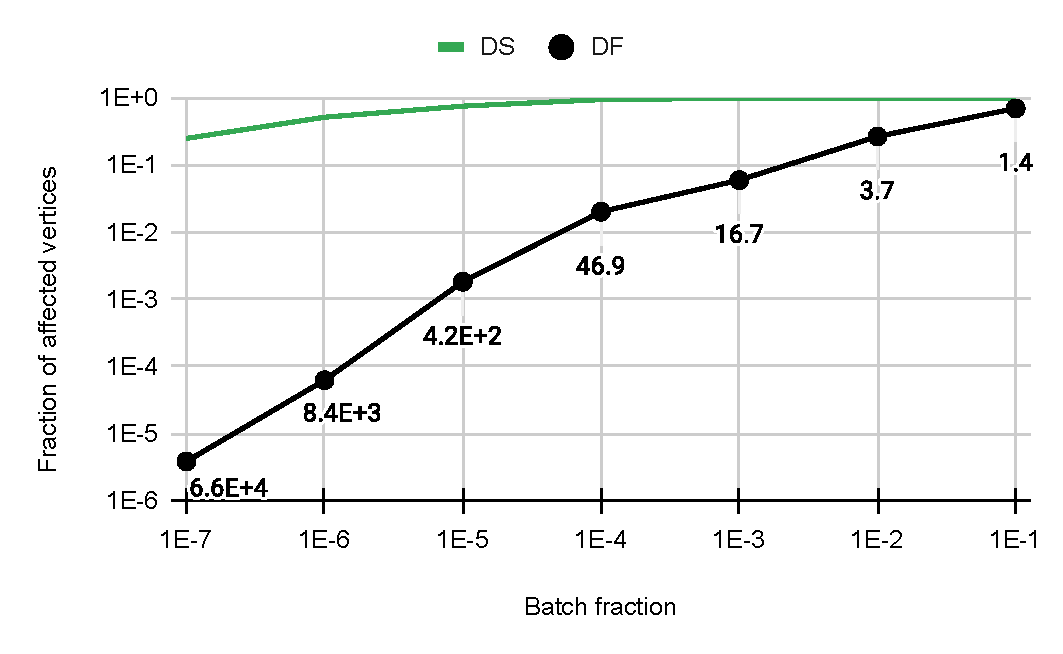
\includegraphics[width=0.48\linewidth]{out/measure-affected-8020.pdf}
  } \\[-2ex]
  \caption{Mean percentage of vertices marked as affected by \textit{Delta-screening (DS)} and our \textit{Dynamic Frontier (DF)} Louvain, on real-world dynamic graphs (with batch updates of size $10^{-5}|E|$ to $10^{-3}|E|$), and on large graphs with random batch updates ($80\%$ edge insertions and $20\%$ edge deletions with batch updates of size $10^{-7}|E|$ to $0.1|E|$).}
  \label{fig:measure-affected}
\end{figure*}
